\documentclass{article}


% if you need to pass options to natbib, use, e.g.:
%     \PassOptionsToPackage{numbers, compress}{natbib}
% before loading neurips_2023


% ready for submission
\usepackage[final]{neurips_2023}


% to compile a preprint version, e.g., for submission to arXiv, add add the
% [preprint] option:
%     \usepackage[preprint]{neurips_2023}


% to compile a camera-ready version, add the [final] option, e.g.:
%     \usepackage[final]{neurips_2023}


% to avoid loading the natbib package, add option nonatbib:
%    \usepackage[nonatbib]{neurips_2023}

\usepackage[utf8]{inputenc} % allow utf-8 input
\usepackage[T1]{fontenc}    % use 8-bit T1 fonts
\usepackage{hyperref}       % hyperlinks
\usepackage{url}            % simple URL typesetting
\usepackage{booktabs}       % professional-quality tables
\usepackage{amsfonts}       % blackboard math symbols
\usepackage{amsmath}
\usepackage{nicefrac}       % compact symbols for 1/2, etc.
\usepackage{microtype}      % microtypography
\usepackage{xcolor}         % colors
\usepackage{graphicx}
\usepackage{float}
\usepackage{subfig}

\bibliographystyle{plainnat}


\title{ECEN 757 | Homework 1}


% The \author macro works with any number of authors. There are two commands
% used to separate the names and addresses of multiple authors: \And and \AND.
%
% Using \And between authors leaves it to LaTeX to determine where to break the
% lines. Using \AND forces a line break at that point. So, if LaTeX puts 3 of 4
% authors names on the first line, and the last on the second line, try using
% \AND instead of \And before the third author name.

\author{%
  Muhammed U. Ersoy\\
  M.S. ECEN Student\\
  Texas A\&M University\\
  \texttt{mue@tamu.edu} \\
 }

\begin{document}
\maketitle
\section{A client attempts to synchronize with a time server. It records the round-trip times and
timestamps returned by the server in the table below.}
\begin{table}[H]
\centering
\begin{tabular}{ll}
\toprule
Round-trip (ms) & Time (hr:min:sec) \\ \midrule
22              & 10:54:23.674      \\
25              & 10:54:25.450      \\
20              & 10.54:28.342      \\ \bottomrule
\end{tabular}
\end{table}

\subsection{Which of these times should it use to set its clock? To what time should it set it?}

Using the simplest form of Cristian's algorithm we can use the third timestamp which was filled by the server
the latest, it has the lowest $T_{round}$ which lowers upper-bound of the inaccuracy.

We should set our clock to;
\begin{equation}
    t + \frac{T_{round}}{2} = \textit{10.54:28.342} + \frac{20}{2} = \textit{10.54:28.352}
\end{equation}
\subsection{Estimate the accuracy of the setting with respect to the server’s clock.}
Since we have no information about the $\min$ delay time in the network, we have to assume that the message
could have been transmitted instantaneously (or negligible time), in this case server would have received the message
and signed it with its' own timestamp at the same time. In other words $t = m_{received}$, and the message would have to be
delivered in $20ms$ then $m_t = t + 20ms$. 

On the other hand the message could have taken `almost` the full $20ms$ to be received by the server, and returned with a timestamp
in `negligible` time. In this case, $m_{t} = m_{received}$. Hence the range for the actual time is $[t, t + T_{round}]$ or for our case
$[\textit{10.54:28.342}, \textit{10.54:28.362}]

The range of the values is $\nicefrac{T_{round}}{2} = \pm 10ms$

\subsection{If it is known that the time between sending and receiving a message in the system concerned is at least 8
ms, do your answers change?}
Yes, then we know that the message must have taken at least 8ms to travel in either direction. Thus, we now know
that the message must have taken at least $8ms$ to return after being signed, hence the minimum value is $\textit{10.54:28.342} + 8ms = \textit{10.54:28.350}$.

And since we know that the message must have taken at least $8ms$ to return the maximum changes to $\textit{10.54:28.342} + 20ms - 8ms = \textit{10.54:28.354}$.
And since the $\min$ delay times are symmetric for recv \& send, our original formula $t + \nicefrac{T_{round}}{2}$ still holds.

This new fact tightened our uncertainty from $\pm 10ms$ to $\pm 2ms$

\section{An NTP server B receives server A’s message at 16:34:23.480, bearing a timestamp of
16:34:13.430, and replies to it. A receives the message at 16:34:15.725, bearing B’s
timestamp, 16:34:25.7. Estimate the offset between B and A and the accuracy of the
estimate.}

\begin{figure}[H]
    \centering
    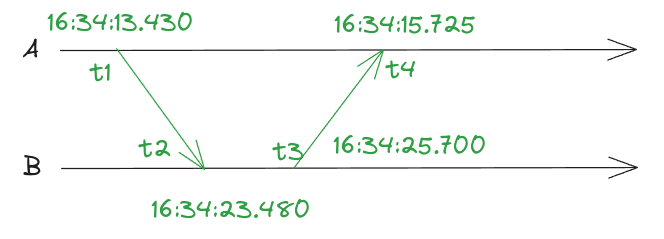
\includegraphics[width=10cm]{q2_fig1.png}
    \caption{Event Flow Of This Transmission}
\end{figure}

In this event graph we have two unknowns, the transmission time, and the offset between the hosts. Let $\triangle t$ be the
offset between the machines, and $T_{t}$ which is a random variable that models the transmission time. Then we can write the following two equations;

\begin{equation}
    \begin{aligned}
        t_2 &= t_1 + T_{t} + \triangle t\\
        t_4 &= t_3 + T_{t} - \triangle t
    \end{aligned}
\end{equation}


We can take the expected value of both sides, and use some algebraic shuffling the variables around to get $\triangle t$ on one side, and the other variables on the other we get the following;

\begin{equation}
    \begin{aligned}
        E[t_2 - t_4] = E[t_1 - t_3 + T_{trans} - T_{trans} + 2\cdot \triangle t] \\
    \end{aligned}
\end{equation}

Since $t_1,t_2,t_3,t_4,\triangle t$ are all constants they can be taken out of the Expected value untouched. 
We can then use the fact that $E[T_t - T_t] = 0$, and get the following equality.
\begin{equation}
    \begin{aligned}
        \triangle t &= \frac{t_2 - t_4 + t_3 - t_1}{2} &= \frac{(t_2 - t_1) + (t_3 - t_4)}{2}
    \end{aligned}
\end{equation}

Based on this the estimated offset between the two hosts is;

\begin{equation}
    \begin{align}
        \frac{(\textit{16:34:23.480}-\textit{16:34:13.430}) + (\textit{16:34:25.700}-\textit{16:34:15.725})}{2}
    = \frac{10.050s + 9.975s}{2} = 10.0125s
\end{align}
\end{equation}

It should be noted that in the previous formula we ignored two uncertainty factors. The first one is the drift that occurs while the messages
are exchanged. This should be fine to ignore as long as the time between messages is small. The second one is when we factored out $E[T_t - T_t]$.
we used a probabilistic outlook that would hold based on the law of large numbers. However in this case we only have 2 samples (transmissions).
Hence, in this case it would be apt to replace $E[T_t - T_t]$ with a term for the uncertainty.

\begin{equation}
    \begin{aligned}
        \triangle t &= \frac{(t_2 - t_1) + (t_3 - t_4)}{2} + O(n)
    \end{aligned}
\end{equation}

We are also assuming both sides of the transmission follow the same distribution. However I'll keep ignoring this since we don't
know anything about the distribution(s) anyways.

Let's take a look at what we can say about the accuracy of this estimate.

If the transmission delay was 0. The minimum offset would be $9.975s$ and the maximum would be $10.050s$. Depending on the transmission
delay the offset could be anywhere in the following range $[9.975s, 10.050s]$. Thus $O(t)$ has a range of $\pm 0.0375s$.

\section{Using the result of Exercise 14.11, show that if events e and e' are concurrent then
neither V(e) $\leq$ V(e') nor V(e') $\leq$ V(e). Hence show that if V(e)< V(e') then e $\rightarrow$ e'.}

\subsection{Let's first prove $V_j[i] \leq V_i[i]$}

Remember that $V_i$ is a logical counter on machine $i$, and $V_j$ is the logical counter on machine $j$.
The $i^{th}$ element of $V_i$ is incremented when an event occurs on $i$. Every time an event communicates with the $j^{th}$ machine
$i^{th}$ element of $V_j$ is synced to $V_i$. Thus $V_j[i] \leq V_i[i]$.

\subsection{$V(e) < V(e') \implies e \rightarrow e'$}

$V(e) < V(e')$ means that every element of $V(e')$ is greater than \textbf{or equal to} $V(e)$ but at least one
element must be \textbf{greater than} $V(e)$.

We can prove this by contradiction. Let $e$ and $e'$ be two succesive events st. $e \rightarrow e'$.
Assume $V(e) > V(e')$.

There are two cases;

The first is that these are events in the same process. This case is really straight forward, $V(e')[i] = V(e)[i] + 1$
thus $V(e) > V(e')$ is a contradiction. We took the same vector and incremented one of its elements. $V(e) < V(e')$ is by definition.

The second case is a cross machine process. In this case we run the following procedure;

\begin{equation}
    \begin{aligned}
        V(e')[i] &:=\max \{ V(e), V(e') \} \forall i \in 0,...,N\\
        V(e')[i] &+= 1 \text{if i == current process} 
    \end{aligned}
\end{equation}

Hencefort, $V(e) < V(e')$ implies $e \rightarrow e'$. And since the this statement is the contrapositive of the statement in the problem definition the proof
is complete.
\section{Two processes P and Q are connected in a ring using two channels, and they constantly
rotate a message m. At any one time, there is only one copy of m in the system. Each
process’s state consists of the number of times it has received m, and P sends m first. At
a certain point, P has the message and its state is 101. Immediately after sending m, P
initiates the snapshot algorithm. Explain the operation of the algorithm in this case,
giving the possible global state(s) reported by it.}

\begin{itemize}
    \item P sends m
    \item P records state (101)
    \item P sends marker
    \item Q receives m, making its state 102
    \item Q receives marker and by marker-receiving rule, records its state (102) and state of the channel from P to Q as {}
    \item Q sends marker
    \item Q sends m again t some point later
    \item P receives marker
    \item P records the state of the channel from Q to P as set of messages received since it saved its state = {}
\end{itemize}

This answer was taken from \citet{grc}.I don't think I quite understood this algorithm well, particularly when it comes to networks
with 3+ machines.

\section{Use the figure right above 14.15, mark the timestamps for both Lamport timestamp and Vector
clock}
\begin{figure}[H]
    \centering
    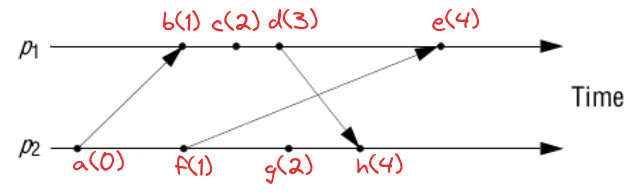
\includegraphics[width=10cm]{lamport.png}
    \caption{Lamport timestamps}
\end{figure}
\begin{figure}[H]
    \centering
    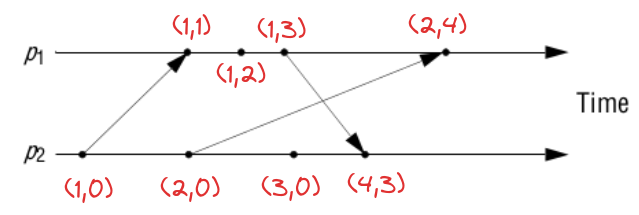
\includegraphics[width=10cm]{vector.png}
    \caption{Vector timestamps}
\end{figure}

\section{Reach out to your partners for your final presentation. Attach
screenshots of your communications.} 
\begin{figure}[H]
    \centering
    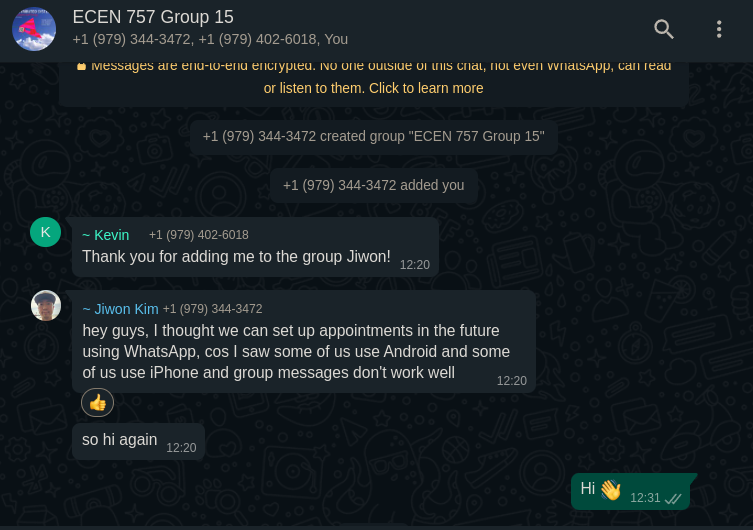
\includegraphics[width=10cm]{com_1.png}
    \caption{Screenshot of Communications}
\end{figure}

\bibliography{default}
\end{document}


